% =============================================================================
% 数学建模竞赛论文通用模板
% 使用 XeLaTeX 编译以支持中文
% =============================================================================

\documentclass[12pt,a4paper]{article}

% ---------- 基础包 ----------
\usepackage{ctex}                                          % 中文支持
\usepackage[margin=2.5cm]{geometry}                        % 页边距
\usepackage{amsmath, amssymb}                              % 数学公式
\usepackage{graphicx}                                      % 插图
\usepackage{csvsimple}                                     % CSV 数据导入
\usepackage{booktabs}                                      % 三线表
\usepackage{float}                                         % 浮动体控制
\usepackage{caption}                                       % 图表标题
\usepackage{subcaption}                                    % 子图
\usepackage{array, multirow}                               % 表格增强
\usepackage{longtable}                                     % 长表格
\usepackage[colorlinks=true,linkcolor=black,urlcolor=blue,citecolor=blue]{hyperref}
\usepackage{fancyhdr}                                      % 页眉页脚
\usepackage{enumitem}                                      % 列表控制

% ---------- 页眉页脚 ----------
\pagestyle{fancy}

\fancyhf{} % 清空默认页眉页脚

\fancyhead[C]{\the\year 年北京理工大学数学建模竞赛}

\fancyfoot[C]{\thepage} % 页脚居中页码

\title{论文标题}
\author{}
\date{}

\fancypagestyle{plain}{
  \fancyhf{}
  \fancyhead[C]{\the\year 年北京理工大学数学建模竞赛}
  \fancyfoot[C]{\thepage}
  \renewcommand{\headrulewidth}{0.4pt}
  \renewcommand{\footrulewidth}{0pt}
}

\renewcommand{\headrulewidth}{0.4pt} % 页眉横线
\renewcommand{\footrulewidth}{0pt}   % 页脚横线
\setlength{\headheight}{14.49998pt}

\begin{document}

% ===== 承诺书 =====
\begin{center}
    {\Large \bfseries 参赛承诺书}
\end{center}

\vspace{1.5em}

\noindent
\textbf{提交包含此承诺书的pdf文件，表明所有此文件的作者共同承诺：}

\medskip

我们完全清楚，在竞赛开始后参赛队员不能以任何方式，包括电话、电子邮件、“贴吧”、QQ群、微信群等，与队外的任何人(包括指导教师)交流、讨论与赛题有关的问题；无论主动参与讨论还是被动接收讨论信息都是严重违反竞赛纪律的行为。

\medskip

\textbf{我们以中国大学生名誉和诚信郑重承诺，严格遵守竞赛章程和参赛规则，以保证竞赛的公正、公平性。如有违反竞赛章程和参赛规则的行为，我们将受到严肃处理。}

\medskip

我们授权北京理工大学数学建模竞赛组织方，可将我们的论文以任何形式进行公开展示(包括进行网上公示，在书籍、期刊和其他媒体进行正式或非正式发表等)。

\begin{flushright}
\the\year.\the\month
\end{flushright}

\newpage % 承诺书单独一页

% =============================================================================
\maketitle

\renewenvironment{abstract}
{\par\noindent}
{\par}
\begin{abstract}
\noindent
\textbf{摘要}：在此处撰写论文摘要，简要介绍问题背景、所用模型与方法、主要结果与结论。摘要应独立成段，涵盖问题的提出、建模思路、关键发现及实际意义，字数控制在 300--500 字左右。

\vspace{0.5em}
\noindent
\textbf{关键词}：关键词1；关键词2；关键词3；关键词4
\end{abstract}

\newpage % 摘要单独一页

% =============================================================================
\section{图表插入示例}
\subsection{图片插入示例}
为...，我们...，如下图(图~\ref{fig:example-png})所示：

\begin{figure}[H]
  \centering
  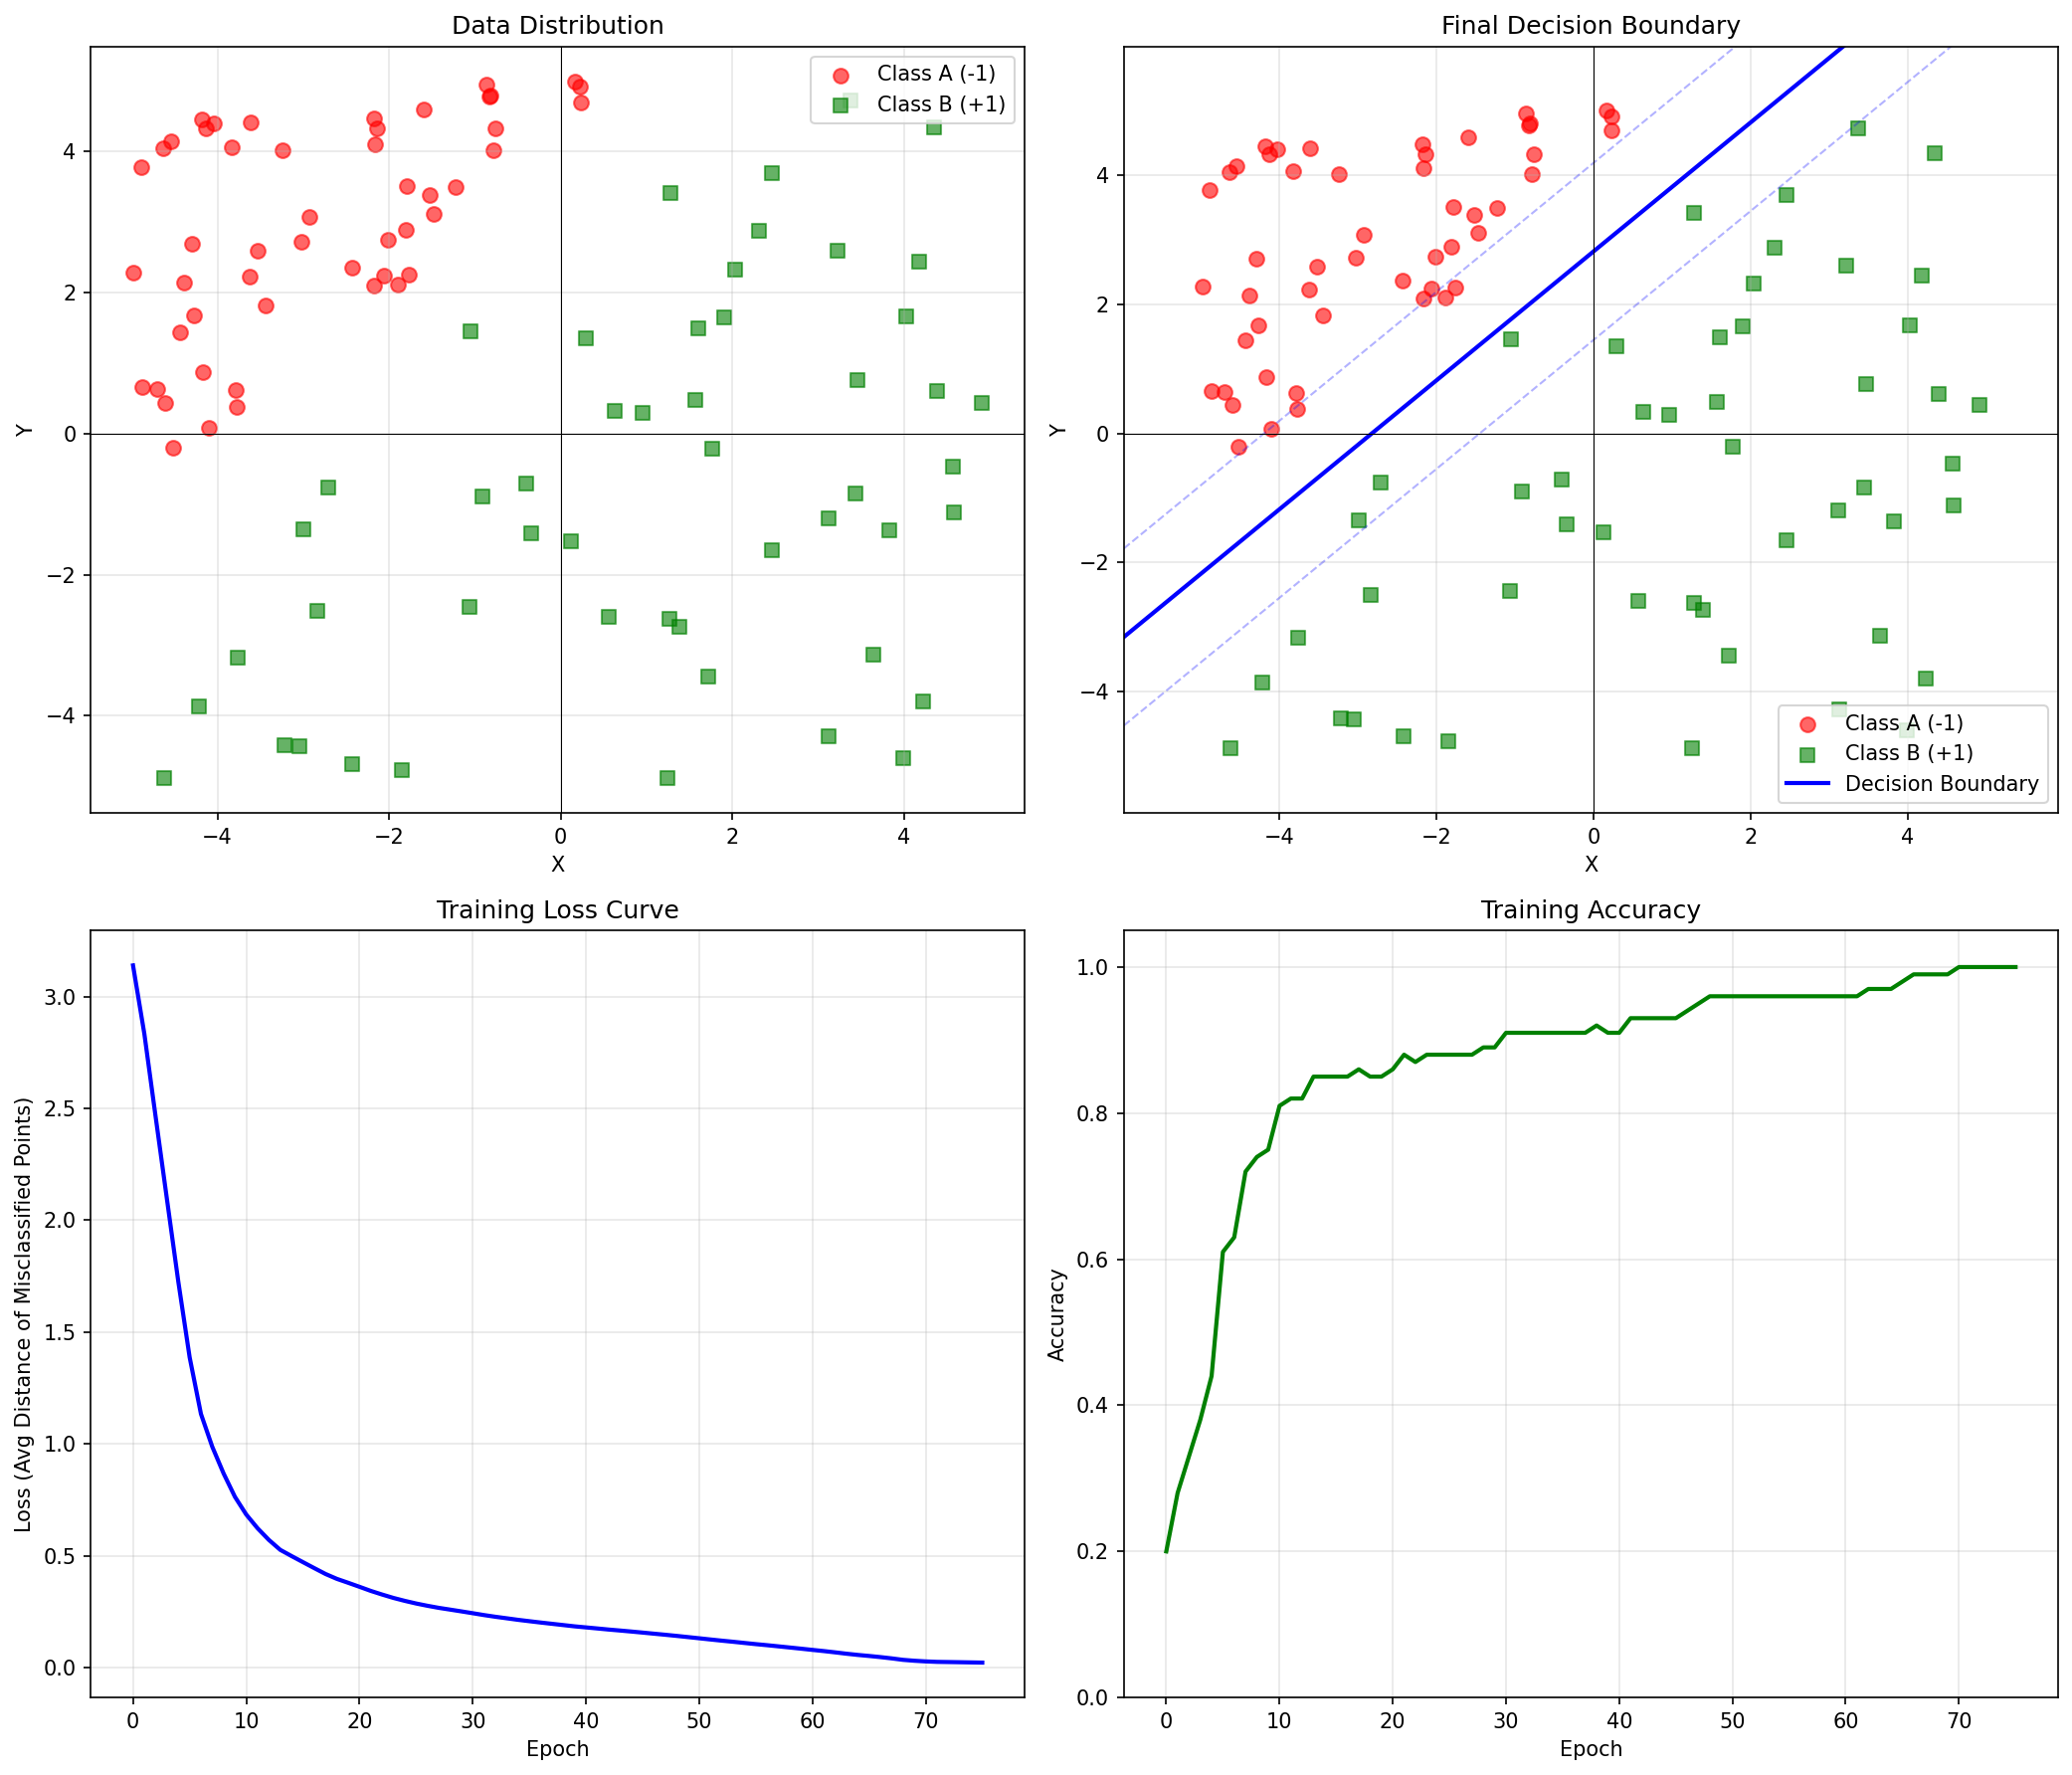
\includegraphics[width=\textwidth]{figs/example.png}
  \caption{示例图片}
  \label{fig:example-png}
\end{figure}

由图~\ref{fig:example-png} 可知...

\subsection{表格插入示例}
为...，我们...，如下表(表~\ref{tab:example-csv})所示：

% 方式一：直接在 LaTeX 中编写表格
\begin{table}[H]
  \centering
  \caption{示例表格（手动编写）}
  \label{tab:example-manual}
  \begin{tabular}{llll}
    \toprule
    Name & Gender & Age & Score\\
    \midrule
    Alice & Female & 20 & 95\\
    Bob & Male & 21 & 88\\
    Charlie & Male & 19 & 92\\
    \bottomrule
  \end{tabular}
\end{table}

% 方式二：从 CSV 文件导入并渲染为三线表
% \csvautobooktabular 自动读取表头 + 三线表样式（toprule/midrule/bottomrule）
\begin{table}[H]
  \centering
  \caption{示例表格（CSV导入）}
  \label{tab:example-csv}
  \csvautobooktabular{tabs/data.csv}
\end{table}

由表~\ref{tab:example-csv} 可知...

% =============================================================================
\section{问题背景}

在此处描述问题的应用背景和实际意义。阐述问题所涉及的领域、核心挑战，以及解决该问题对相关领域或实际应用的推动作用。可引用已有研究来说明问题的重要性和现有方法的局限性，引出本文的研究动机。根据需要可添加引用 \cite{ref1}。

% =============================================================================
\section{问题分析}

\subsection{问题整体结构}

在此处分析各子问题之间的逻辑关系：哪些是递进的、哪些是并列的、哪些依赖于前面问题的结果。用简短的文字勾勒出建模的整体路线图。

\subsection{关键难点分析}

在此处指出每个子问题的核心挑战，以及建模时需要解决的主要矛盾（如精度与可解释性的权衡、计算效率、数据稀疏性等）。

% =============================================================================
\section{模型基本假设}

在此处列出适用于全文的通用假设。每条假设应说明其依据以及适用范围。

\begin{itemize}
    \item \textbf{假设1名称}：假设1的详细描述与依据。
    \item \textbf{假设2名称}：假设2的详细描述与依据。
    \item \textbf{假设3名称}：假设3的详细描述与依据。
\end{itemize}

% =============================================================================
\section{数据预处理与特征工程}

\subsection{原始数据清洗}

在此处描述数据清洗过程，包括缺失值处理、异常值检测与修正、重复记录删除等步骤，并说明清洗后的数据规模与质量。

\subsection{补充数据}

如需引入外部数据源作为补充，在此处说明数据来源、获取方式、变量含义及预处理步骤。

\subsection{特征工程}

在此处描述特征构造过程，包括时间特征、滞后特征、交叉特征、耦合特征等的构造方法及最终特征维度。

% =============================================================================
\section{问题一模型构建与求解}

\subsection{问题一分析}

在此处对问题一进行针对性分析。说明选择当前建模方法的原因，以及相对于通用假设需要补充哪些假设。

\subsection{问题一补充假设}

\begin{itemize}
    \item \textbf{补充假设1}：假设内容与依据。
    \item \textbf{补充假设2}：假设内容与依据。
\end{itemize}

\subsection{模型建立}

在此处详细描述模型的数学形式。使用 \texttt{equation} 环境对核心公式进行编号，并解释每一项的物理或统计含义。如涉及算法，可用伪代码或流程图辅助说明。

\subsection{模型求解}

在此处说明求解方法：解析解推导过程，或数值求解算法及其参数设置。对需要调参的方法，给出参数选取准则。

\subsection{结果与分析}

在此处展示问题一的计算结果，用图表和文字概括关键发现。图表需有清晰的标题和坐标轴标注。

% =============================================================================
\section{问题二模型构建与求解}

\subsection{问题二分析}

在此处分析问题二与问题一的联系与区别，说明建模思路的调整和新增考虑的因素。

\subsection{问题二补充假设}

\begin{itemize}
    \item \textbf{补充假设1}：假设内容与依据。
    \item \textbf{补充假设2}：假设内容与依据。
\end{itemize}

\subsection{模型建立}

在此处详细描述模型。

\subsection{模型求解}

在此处说明求解方法与计算过程。

\subsection{结果与分析}

在此处展示结果并进行讨论。

% =============================================================================
\section{问题三模型构建与求解}

\subsection{问题三分析}

在此处分析问题三与前面问题的关系，说明整体链路和建模思路。

\subsection{问题三补充假设}

\begin{itemize}
    \item \textbf{补充假设1}：假设内容与依据。
    \item \textbf{补充假设2}：假设内容与依据。
\end{itemize}

\subsection{模型建立}

在此处详细描述模型。

\subsection{模型求解}

在此处说明求解方法与计算过程。

\subsection{结果与分析}

在此处展示结果并进行讨论。

% =============================================================================
\section{模型评价与改进}

\subsection{模型优点}

\begin{enumerate}
    \item 优点1：简要描述。
    \item 优点2：简要描述。
    \item 优点3：简要描述。
\end{enumerate}

\subsection{模型局限性}

\begin{enumerate}
    \item 局限性1：简要描述，说明对结果的影响。
    \item 局限性2：简要描述，说明对结果的影响。
    \item 局限性3：简要描述，说明对结果的影响。
\end{enumerate}

\subsection{改进方向}

\begin{enumerate}
    \item 改进方向1：简要描述改进思路及预期效果。
    \item 改进方向2：简要描述改进思路及预期效果。
    \item 改进方向3：简要描述改进思路及预期效果。
\end{enumerate}

% =============================================================================
\section{总结}

在此处用条目列表概括论文的主要工作与核心结论。每条结论应精炼，突出创新点和关键数据。

\begin{enumerate}
    \item 结论1：简要描述。
    \item 结论2：简要描述。
    \item 结论3：简要描述。
    \item 结论4：简要描述。
\end{enumerate}

% =============================================================================
\section{参考文献}

\begin{thebibliography}{99}

\bibitem{ref1}
作者1, 作者2. 论文标题. \textit{期刊名称}, 年份, 卷(期): 页码.

\bibitem{ref2}
作者1, 作者2. 论文标题. \textit{期刊名称}, 年份, 卷(期): 页码.

\bibitem{ref3}
作者1, 作者2. 论文标题. \textit{期刊名称}, 年份, 卷(期): 页码.

\end{thebibliography}

% =============================================================================
\section{附录}

在此处放置正文中不宜展开但有必要留存的内容：代码清单、数据表格、补充推导、算法伪代码等。

\subsection{代码模块}

\begin{itemize}
    \item \texttt{module\_1.py}：模块功能简要说明。
    \item \texttt{module\_2.py}：模块功能简要说明。
\end{itemize}

\subsection{补充数据与图表}

在此处放置额外的数据表、中间结果或补充图表。

\end{document}
